\documentclass[12pt]{exam}
\usepackage[utf8]{inputenc}
\usepackage{fancyvrb}
\usepackage{ngerman}
\usepackage{graphicx}
\usepackage{color}
\usepackage{listings}
\usepackage{eurosym}
%new commands
\newcommand{\klausurart}{Klausur}
\newcommand{\thema}{Programmierparadigmen (A107)}
\newcommand{\zenturie}{A14}
\newcommand{\klausurtag}{13.10.2017}
\newcommand{\quartal}{(3/2017)}
\newcommand{\klausurdauer}{90}
\newcommand{\hilfsmittel}{Keine (auch kein Taschenrechner)}
\newcommand{\pruefung}{Bachelor Angewandte Informatik}
\newcommand{\dozent}{J. Brauer}
%page formating
\parindent0pt
\parskip4mm plus 2mm minus 1mm
\lhead{\dozent}
\chead{
\includegraphics[scale=0.15]{hochs.png} }
\rhead{\klausurtag}
\cfoot{\klausurart \ \thema \ Seite \thepage \ von \numpages}

\renewcommand\thepartno{\arabic{question}.\arabic{partno}}
\pointpoints{Punkt}{Punkte}
\addpoints
\qformat{\textbf{Aufgabe} \thequestion \ (\pointsofquestion{\arabic{question}} \points )\hfill}
\shadedsolutions
\definecolor{SolutionColor}{rgb}{1,1,0.7}
\renewcommand{\solutiontitle}{\noindent \textbf{Lösung:} \par \noindent}
\setlength\linefillheight{1cm}

%\printanswers
\begin{document}
\begin{coverpages}

\hbox to 16.5cm{\hbox to 6cm{\vbox{\dozent}}\hfill\hbox to 10.5cm{\hfill
\includegraphics[scale=0.4]{hochs.png}}}



\begin{center}
\Large \bf{\klausurart\ \thema 

Quartal: \quartal}
\end{center}
\vspace{0.3cm}
\hbox to 16.5cm{\hbox to 9cm{\textbf{Name des Prüflings:}  \hfill}
\vspace{0.6cm}
\hbox to 5cm{\textbf{Matrikelnummer: }  \hfil}\hbox to 2.5cm{\textbf{Zenturie:}  \hfil}}

%\vspace{1cm}
\hbox to 16.5cm{\hbox to 7.5cm{ \hrulefill}\hfil\hbox to 3.8cm{\hrulefill}\hfil\hbox to 2.5cm{ \hrulefill}}

\vspace{0.3cm}
Dauer: \klausurdauer \,Min. \hfill Seiten der \emph{Klausur} \textbf{ohne} Deckblatt: \numpages
\hfill Datum: \klausurtag

\vspace{0.7cm}

\begin{tabular}{p{6cm}p{9.5cm}}

Hilfsmittel: &
\begin{itemize}
%  \item NAK Taschenrechner
  \item \hilfsmittel
\end{itemize}\\

Bemerkungen: &
\begin{itemize}
  \item \textbf{Bitte prüfen Sie zunächst die Klausur \mbox{(alle Teile)} auf Vollständigkeit.}
  \item \textbf{Bitte lösen Sie nicht die Heftung.}
\end{itemize}\\
\end{tabular}

Es sind 90 Punkte erreichbar!\par
Zum Bestehen der Klausur sind 45 Punkte ausreichend!

\begin{center}
\hqword{Aufgabe:}
\htword{Summe:}
\hsword{Erreichte Punkte:}
\hpword{Erreichbare Punkte:}
\cellwidth{2.2em}
\gradetable[h]
\end{center}

\vspace{0.5cm}

\enlargethispage{2cm}

\hbox to 16.5cm {
  \hbox to 3cm{Note: \enspace \hrulefill}\hfill
  \hbox to 4cm{Prozentsatz: \enspace \hrulefill}\hfill
  \hbox to 6cm{Ergänzungsprüfung: \enspace \hrulefill}}

\vspace{0.8cm}
\hbox to 16.5cm {
  \hbox to 4cm{Datum: \enspace \hrulefill}\hfill
  \hbox to 10cm{Unterschrift: \enspace \hrulefill}}

% \vspace{0.8cm}
% \hbox to 16.5cm {
% \hbox to 4cm{Datum: \enspace \hrulefill}\hfill
% \hbox to 10cm{Unterschrift: \enspace \hrulefill}}

\end{coverpages}

\begin{questions}

\question[8]
\vspace{0.5cm}


\begin{tabular}{|l|p{10cm}|c|p{1.8 cm}|}
    \hline
    &Beantworten Sie die folgenden Fragen:&stimme zu&stimme nicht zu \\
    \hline
    
a)&Zuweisungen an Variablen stellen 
ein bedeutendes Ausdrucksmittel der funktionalen Programmierung dar.&&\\
\hline


b)&Funktionen, die Argumente akzeptieren, bezeichnet man als
    Funktionen höherer Ordnung.&&\\
\hline

c)&Rekursive Funktionen sind notwendig immer auch bedingte Funktionen.&&\\
\hline

d)&Ein Merkmal der Entwurfsvorschriften besteht in der Ableitung
der Funktionsschablone aus der Struktur der zu verarbeitenden Daten.&&\\
\hline

e)&Die Zeit, die ein Programmierer benötigt, um eine Zeile Code zu
  schreiben, ist eine Konstante (unabhängig von der Programmier\-sprache).&&\\
\hline

f)&In funktionalen Sprachen mit strikter Auswertungsstrategie dienen
    thunks dazu, verzögerte Auswertung zu erreichen&&\\
\hline

g)&Das Ersetzungsmodell für Funktionsanwendungen ist auch auf
    zustandsbehaftete Prozeduren übertragbar.&&\\
\hline

h)&Logische Programme bestehen aus Fakten, Regeln und Variablenzuweisungen.&&\\
\hline

\end{tabular}

Jede richtige Antwort wird mit je 1 Punkt, jede falsche oder nicht
gegebene Antwort mit 0 Punkten bewertet.

\pagebreak

\question[4]
Ein fundamentales Prinzip der funktionalen Programmierung lautet:
\begin{center}
Funktionen sind Werte erster Ordnung. 
\end{center}
Was folgt aus diesem Prinzip für die Verwendung von Funktionen?

\pagebreak

\question

Für die folgenden Ausdrücke bzw. Ausdruckssequenzen geben Sie jeweils
Wert und Typ des Ergebnisses an, das sich aus der Auswertung des
jeweils letzten Ausdrucks ergibt. Sie brauchen nur die Endergebnisse
-- nicht deren Ableitung -- angeben. 
Für den \textbf{Typ} des Ergebnisses
genügen Angaben wie "`Zahl"', "`Symbol"' oder dergleichen. Falls es
sich beim Ergebnis um eine primitive (eingebaute) Funktion handelt,
schreiben Sie als Wert "`primitive Funktion"', falls es sich um eine
benutzerdefinierte Funktion handelt, schreiben Sie einfach
"`Funktion"'. Für den \textbf{Typ} einer Funktion geben Sie den
\textbf{Vertrag} in informeller Notation (z.\,B. \texttt{(list-of any)
  -> boolean}) an.

Beispiele: 

  \begin{tabular}{|l|l|l|}
  	\hline
    \textbf{Ausdruck}&\textbf{Wert}&\textbf{Typ}\\
    \hline
    \texttt{(> 4 5)}&\texttt{false}&\texttt{Boolean}\\
    \hline
    \texttt{(fn [x] (* x x)}&\texttt{Funktion}&\texttt{Zahl -> Zahl}\\
    \hline
  \end{tabular}

Hinweis: \textbf{Alle Ausdrücke lassen sich ohne Fehler auswerten.}


\begin{parts}
  \part[2] \ 
  \begin{verbatim} 
(def + -) 
(def / *) 
(+ 15 (/ 2 7)) 
\end{verbatim}

\vspace{0.5cm}
Wert:\begin{solution}1\end{solution}

\vspace{0.5cm}
Typ:
\vspace{0.5cm}
\part[3] \ 
\begin{verbatim}
(def a 15) 
(def b 'x)
(def f
  (fn [a]
    (let [b 1]
      (- a b))))
(f 2)
\end{verbatim}

\vspace{0.5cm}
Wert: \begin{solution}1\end{solution}

\vspace{0.5cm}
Typ:
\vspace{0.5cm}

\part[4] \ 
  \begin{verbatim}
((fn [x + y] (+ x y)) 5 - 4)
\end{verbatim}

\vspace{0.3cm}
Wert: \begin{solution}1\end{solution}

\vspace{0.3cm}
Typ:

\pagebreak
\part[5] \
\begin{verbatim}
((fn [x]
   (fn [y]
     (+ (Math/sin x) (Math/cos y))))
 3.14159)
\end{verbatim}

\vspace{0.5cm}
Wert: \begin{solution}Funktion\end{solution}

\vspace{0.5cm}
Typ: \begin{solution}Zahl -> Zahl\end{solution}
\vspace{0.5cm}
\end{parts}


\pagebreak
\question[12]
Was ist der Wert des letzten Ausdrucks in folgendem Programm? Begründen Sie Ihre Antwort z.\,B. durch Anwendung des Ersetzungsmodells.
\begin{verbatim}
(def schnittchen 41)
(def canapee 43)

(def haeppchen
  (fn [schnittchen canapee]
    ((fn [schnittchen]
       (- schnittchen canapee))
     schnittchen)))

(haeppchen canapee schnittchen)
\end{verbatim}

\pagebreak

\ 

\pagebreak

\question
\begin{parts}
  \part[5]Entwickeln Sie die folgende Funktion unter Anwendung der
  Entwurfsvorschrift III:

  Die Funktion \texttt{memrest} liefere, angewendet auf ein Symbol
  \texttt{sym} und eine Liste von Symbolen \texttt{lvs}, die Teilliste
  von \texttt{lvs}, die mit dem erstmaligen Auftreten von \texttt{sym}
  in \texttt{lvs} beginnt. Kommt \texttt{sym} in \texttt{lvs} nicht
  vor, ist das Ergebnis die leere Liste. 

Beispiele:
    
  \verb|(memrest 'a '(x y z)) ==> '()|

  \verb|(memrest 'a '(x a y a z)) ==> '(a y a z)|

  Geben Sie alle Bestandteile von Entwurfsvorschrift III an.

  \part [9] Schreiben Sie eine Funktion \texttt{skelett}, die
  ermittelt, ob eine Liste \texttt{skl} ein Skelett einer anderen Liste
  \texttt{lst} ist. Eine Liste \texttt{skl} ist genau dann ein Skelett
  einer Liste \texttt{lst}, wenn durch Entfernung beliebiger Elemente
  aus \texttt{lst} die Liste \texttt{skl} entsteht. Mit anderen Worten:
  Die Elemente von \texttt{skl} kommen in der Reihenfolge, in der sie in
  \texttt{skl} auftreten, auch in \texttt{lst} vor.

  Im einzelnen gelten folgende Aussagen:

  \begin{enumerate}
  \item Die leere Liste ist Skelett jeder anderen Liste
    (einschließlich der leeren Liste): \texttt{(skelett '() l)}
    liefert \texttt{true}.
  
  \item Eine nicht-leere Liste ist niemals Skelett einer leeren Liste:

    \texttt{(skelett '(a b x) '())} liefert \texttt{false}.

  \item Falls \texttt{(first skl)} in \texttt{lst} vorkommt, dann ist
    \texttt{skl} genau dann ein Skelett von \texttt{lst}, wenn
    \texttt{(rest skl)} ein Skelett der Teilfolge von \texttt{lst} ist, die
    hinter dem ersten Vorkommen von \texttt{(first skl)} in \texttt{lst}
    beginnt. Beispiele:

    \verb+(skelett '(a b c ) '(x a a y b c z)) ==> true+

    \verb+(skelett '(a b c d) '(x a a y b c z)) ==> false+

  \end{enumerate}

\textbf{Hinweise}:
\begin{enumerate}
\item Sie brauchen nur die reine Funktionsdefinition aufschreiben. 
\item Es ist zweckmäßig, für die Funktion \texttt{skelett} die
  Funktion \texttt{memrest} aus Teil 1 der Aufgabe zu benutzen. Dafür
  dürfen sie voraussetzen, dass die Listen nur Symbole enthalten.
\end{enumerate}
\end{parts}
\pagebreak
\ 

\pagebreak
\ 

\pagebreak
\ 
\pagebreak
\ 

\question

\begin{parts}
    \part[4] Die Funktion
\begin{verbatim}
(def zahlenfolgeaufwaerts
  (fn [z1 z2]
    (cond 
      (> z1 z2) '()
      :else (cons z1 (zahlenfolgeaufwaerts (+ z1 1) z2 )))))
\end{verbatim}
liefert, 
    angewendet auf zwei natürliche Zahlen $z1$ und $z2$, eine Liste mit den
    ganzen Zahlen aus dem Intervall $z1$ bis $z2$
    (einschließlich). Falls $z1$ größer als $z2$ ist, ist die leere
    Liste das Resultat.
Beispiele:
    
    \verb|(zahlenfolgeaufwaerts 10 16) ==> (10 11 12 13 14 15 16)|
    
    \verb|(zahlenfolgeaufwaerts 3 3)   ==> (3)|

    \verb|(zahlenfolgeaufwaerts 4 3)   ==> ()|

Schreiben Sie eine zweite Funktion, mit Namen
\texttt{zahlenfolgeabwaerts}, die ein absteigendes Zahlenintervall
erzeugt. Beispiele:

    \verb|(zahlenfolgeabwaerts 9 7) ==> (9 8 7)|
    
    \verb|(zahlenfolgeabwaerts 3 3)   ==> (3)|

    \verb|(zahlenfolgeabwaerts 3 4  ==> ()|

\textbf{Hinweis}: Sie brauchen nur die Funktionsdefinition aufschreiben.

    \part[6] Abstrahieren Sie die beiden Funktionen
    \texttt{zahlenfolgeaufwaerts} und
    \texttt{\texttt{zahlenfolgeabwaerts}} zu einer Funktion
    (\texttt{zahlenfolge}) höherer Ordnung, mit der auf- und
    absteigende Zahlenfolgen erzeugt werden können.

\textbf{Hinweis}: Sie brauchen nur die Funktionsdefinition aufschreiben.
    \part[2] Geben Sie den Vertrag von \texttt{zahlenfolge} an.
    
\pagebreak
\ 

\pagebreak
\ 

\end{parts}

\question[10]
Gegeben sei folgende Funktion:
\begin{verbatim}
(def f
  (fn [n]
    (cond
     (= n 1) 1
     :else (+ (* n n) (f (- n 1))))))
\end{verbatim}
Beweisen Sie mittels rekursiver Induktion, dass der Aufruf \verb|(f n)| für jede natürliche Zahl $n>0$ 
den Wert
\[f(n)=\sum_{i=1}^{n}i^{2}\]
liefert.

\pagebreak
\  

\pagebreak

\question Die Software-Gleichung von Larry Putnam beschreibt den
phänomenologischen Zusammenhang zwischen der Produktgröße $G$
(gemessen in \emph{lines of code}), dem Aufwand $A$ (gemessen in
Personenstunden), einem Technologiefaktor $P$ und der Projektdauer
$t$:
$$ G = P \cdot A^{\frac{1}{3}} \cdot  t^{\frac{4}{3}}$$ 

Entwickeln Sie eine Lösung dieser Gleichung mithilfe des aus Vorlesung
bekannten Constraint-Programming-Systems. Die Existenz der
Basis-Bausteine für die Addition, Multiplikation und Potenzbildung
darf vorausgesetzt werden.

\begin{parts}
\part [6]

Implementieren Sie die Gleichung als Schaltbild aus den CPS-Grund\-elementen.

\part[4]

Setzen Sie diese Schaltbild in eine Scheme-Prozedur um.
\end{parts}

\pagebreak 
\ 

\pagebreak
\ 

\pagebreak
\ 

\question 
Sie kennen die hölzernen, russischen Puppen -- auch Babuschkas genannt
--, die sich aufgrund ihrer unterschiedlichen Größe ineinander stecken
lassen, wie in der folgenden schematischen Darstellung zu erkennen
ist:

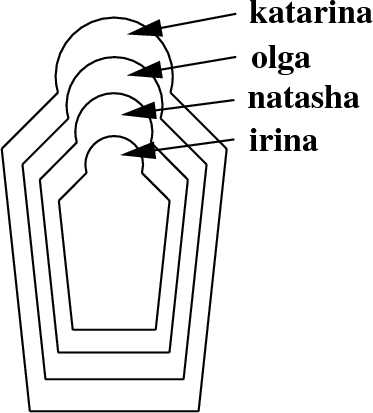
\includegraphics[scale=0.3]{babuschkas.png}

Schreiben Sie folgendes Prolog-Programm:
\begin{parts}
  \part[2]
  Formulieren Sie eine Faktenbasis unter Verwendung eines Prädikats
  \texttt{directlyIn/2}, mit dem beschrieben wird, welche Puppe sich
  direkt in einer anderen Puppe befindet. Benutzen Sie die Babuschkas
  aus der Abbildung.
  \part[4]
  Definieren Sie ein Prädikat \texttt{in/2}, das \texttt{true}
  liefert, wenn sich eine Puppe innerhalb einer anderen (direkt oder
  indirekt) befindet. Dieses Prädikat ist so zu schreiben, dass es
  auch für andere Babuschka-Konstellationen funktioniert.
\end{parts}

\begin{solution}
  directlyIn(katarina, olga).  directlyIn(olga, natsha).
  directlyIn(natsha, irina).

  in(X,Y) :- directlyIn(X,Y).  in(X,Y) :- directlyIn(X,Z), in(Z,Y).
\end{solution}
\pagebreak
\ 
\end{questions}

\end{document}